\documentclass[a4paper,USenglish]{lipics}

\usepackage{amssymb}
\usepackage{amsmath}
\usepackage{stmaryrd}
%\usepackage{pst-all}
\usepackage{graphicx}
\usepackage[all]{xy}
\usepackage{fancyvrb}



\usepackage{multirow}
\begin{document}

\title{FLIF: Free Lossless Image Format based on MANIAC Compression}

\author[1]{Jon Sneyers}
\author[2]{Pieter Wuille}
\affil[1]{jon.sneyers@gmail.com}
\affil[2]{pieter.wuille@gmail.com}



\maketitle

\begin{abstract}
We present a new lossless image compression algorithm.
It achieves better compression than popular lossless image formats like PNG and lossless JPEG 2000.
Existing image formats have specific strengths and weaknesses: e.g. JPEG works well for photographic material,
PNG works well for line drawings, especially if there are few distinct colors.
Our method has two main advantages: 1) It does not require the user to know anything about the nature
of the image and choose between image formats accordingly, since for any kind of image,
our method performs as good or better than any of the existing image formats for lossless compression;
2) It supports progressive decoding with little overhead, which makes the format very suitable for responsive web design.
\end{abstract}


\section{Introduction}

It is very annoying to receive image files that are encoded using a non-suitable compression algorithm.
For instance, the image shown in Fig.~\ref{fig:Circos} is 4000 by 4000 pixels (16 megapixels) and takes about
46 megabytes when stored in raw RGB. If the user is sufficiently well informed, she will notice
that this is in fact a line drawing that uses very few different colors (28 to be precise),
so she saves the image as a palette-indexed GIF file of 1106 kilobytes or a PNG file of 804 kilobytes,
and perhaps she even uses a tool like {\tt pngcrush} to further reduce the size of the PNG file by a few kilobytes, or
the newer format WebP in lossless mode to get a 787 kilobytes WebP file.
If the user is not so well informed, he might save the image as a truecolor PNG file
of about 1.5 megabytes, or much worse, as a lossy JPEG file of 5.4 megabytes, a lossy (!) WebP file of
2.4 megabytes, or a lossless JPEG 2000 file of 12 megabytes.

Progressive decoding allows viewers to render a lower-quality preview while the compressed image
stream is loading. This is particularly useful in low-bandwidth conditions.
PNG and GIF support progressive decoding as an option, using interlacing.
The interlacing of GIF happens only in the vertical direction, while PNG uses ``Adam7'' interlacing
which works in two dimensions. However, this interlacing comes at a cost:
in the case of GIF the file size goes up from 1106 kilobytes to 1122 kilobytes (an acceptable increase, but
then again, GIF's interlacing is rather primitive); in the case of PNG, the file size increases
more dramatically, from 802 kilobytes to 1146 kilobytes.


\begin{figure}
\begin{center}
\begin{minipage}[b]{0.7\textwidth}
\includegraphics[width=\textwidth]{images/Circos}
\end{minipage}
\end{center}
\caption{ The image {\tt Circos.ppm} from Niels Fr\"ohling's test set of paletted images.}
\label{fig:Circos}
\end{figure}

Using our image format (which we call FLIF\footnote{FLIF is an abbreviation for ``Free Lossless Image Format''.}),
the file size is reduced to 432 kilobytes, with lossless compression and progressive decoding (interlacing).
To emphasize the point, Fig.~\ref{fig:Circos_artefacts} shows
what (a fragment of) the image looks like when you want to get a similar compression ratio
using (lossy) JPEG, JPEG 2000, or WebP.

\begin{figure}
\begin{minipage}[b]{0.25\textwidth}
Original image\\
= 432K FLIF-file:\\
\includegraphics[width=0.95\textwidth]{images/c_orig}
\end{minipage}%
\begin{minipage}[b]{0.25\textwidth}
357K JPEG file:\\
\includegraphics[width=0.95\textwidth]{images/c_jpeg}
\end{minipage}%
\begin{minipage}[b]{0.25\textwidth}
368K JP2 file:\\
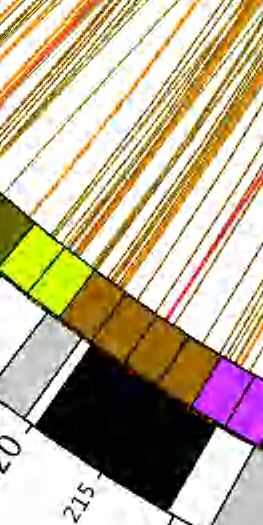
\includegraphics[width=0.95\textwidth]{images/c_jp2}
\end{minipage}%
\begin{minipage}[b]{0.25\textwidth}
422K WebP file:\\
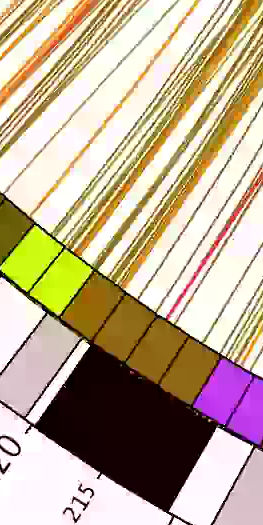
\includegraphics[width=0.95\textwidth]{images/c_webp}
\end{minipage}
\caption{ Fragment of the image {\tt Circos.ppm} which was compressed to about 400 KB using different compression methods.}
\label{fig:Circos_artefacts}
\end{figure}


Image formats like JPEG (2000), or WebP and BPG in lossy mode, are great for compressing photographs, but for other kinds of images,
the compression artifacts can be very visible. Image formats like GIF and PNG work well for line drawings,
but they only support lossless compression (and in the case of GIF, only 256 colors).

If, at the same time, 1) the image clearly fits into one of these two categories (photograph / line drawing), and 2) the user is
sufficiently aware of the properties of the different image formats, 3) the user has the freedom to choose the format,
and 4) a single quality setting suffices for all use cases of the image,
then the existing formats are ``good enough'' in practice. However, these four conditions often do not hold:
\begin{enumerate}
\item Many images are not photographs, nor line drawings, but rather something in between. For example, think of a poster that
contains a photo combined with text elements, or the front page of a newspaper, or a satelite image of the world annotated with labels,
or a screenshot of a web browser. In these cases, the choice between, say, JPEG and PNG is hard: the artifacts of JPEG compression will
be visible, while the PNG file could be too large (e.g. on the web, given limited bandwidth).

\item It is not straightforward to explain to non-technically oriented users when to use which image format (and which compression parameters).
From the point of view of user-friendliness, it does not make sense that the user should worry about the ``internal representation'' of her images.

\item Many devices, applications, and web services only support one or a few image formats. For this reason, sometimes the user is forced
to use a non-suitable image format.

\item Lossy compression by definition means that information is lost, and it is the producer of the image who has to decide how much information
gets lost. However, it is the consumer of the image who knows best what level of information loss is ``acceptable'' for their intended
use of the image.
\end{enumerate}

We believe that the image format we propose in this paper, which is called ``FLIF'', can potentially improve the situation.
New formats have been proposed in the past, but while improving the compression ratio, they kept the distinction between the
two ``categories'' of images largely intact: e.g. JPEG 2000, WebP and BPG improve upon JPEG, and PNG improves upon GIF, but the dichotomy remains
--- in practice, at least two image formats are used and needed (e.g. on the web, JPEG and PNG are currently standard).
FLIF not just improves the compression ratio, but it also makes the old dichotomy obsolete:
FLIF works well for photographs {\em and} for line drawings, and everything ``in between''.



\subsection{Algorithm Overview}

The first step of the encoding algorithm is to convert the image from the RGB(A) color space
to a YIQ(A) color space (in a lossless way) in order to decorrelate the color channels.
It also records which colors actually occur, and decides how much of that color information to store in the encoded file.
Section~\ref{sec:color} discusses this first step.

Next, the image is traversed in some order, and the visited pixels are outputted.
Instead of outputting the actual pixel values, the differences between the predicted values
and the actual values are outputted. The aim is to output smaller numbers; the compression will favor numbers close to zero.
In Section~\ref{sec:traversal} the traversal orders and the prediction methods are introduced.


The pixel difference values are outputted using a sophisticated variant of
context adaptive binary arithmetic coding, called MANIAC. It is ``meta-adaptive'': instead of having a fixed, static
number of contexts (like in FFV1), we use ``dynamic'' contexts that are ``learned'' on the fly.
In this way, only those properties are used that are relevant for the specific image,
resulting in better compression.
In Section~\ref{sec:rac} we discuss the MANIAC entropy encoding mechanism.


The context trees learned during encoding are part of the encoded stream.
This means the decoder can use mostly static contexts, which are less computationally demanding.
The decoding algorithm reconstructs the YIQ image and then converts it back to RGB.

Section~\ref{sec:benchmarks} discusses benchmark results that compare our method with other methods.
Finally, we conclude in Section~\ref{sec:conclusion} with a summary of our contributions and directions for future work.


\section{Color}
\label{sec:color}

In our current implementation,
we assume a source image with integer RGB(A) colors and at most 16 bit depth per color channel.
Our method can be extended to higher bit depths, floating-point pixel values and extra channels.



\subsection{Color Decomposition}

The RGB color representation is well suited for image display on a computer screen, but it does not
match the properties of the human eye. Perceptually, luminosity (essentially the grayscale version of the image)
is more important than color.
% the sentence below is probably biologically not very accurate:
%The human eye has two types of photoreceptors:
%many sensitive rod cells that give a high-resolution grayscale image,
%and relatively few, less sensitive cone cells that give a low-resolution color image.

For lossy image compression it makes sense to take the properties of the human eye into account,
since the aim is to minimize the perceptual error. For this reason, nearly all lossy image
compression algorithms use a different color representation than RGB, and they often use chroma subsampling
and/or quantization.
For lossless compression, it can help to use a different color space to decrease the correlation (and hence redundancy)
between the color planes. Also, while lossless compression by definition has no error,
the perceptual error still matters for progressive decoding.

\begin{figure}
\begin{minipage}[b]{0.25\textwidth}
Original image:\\
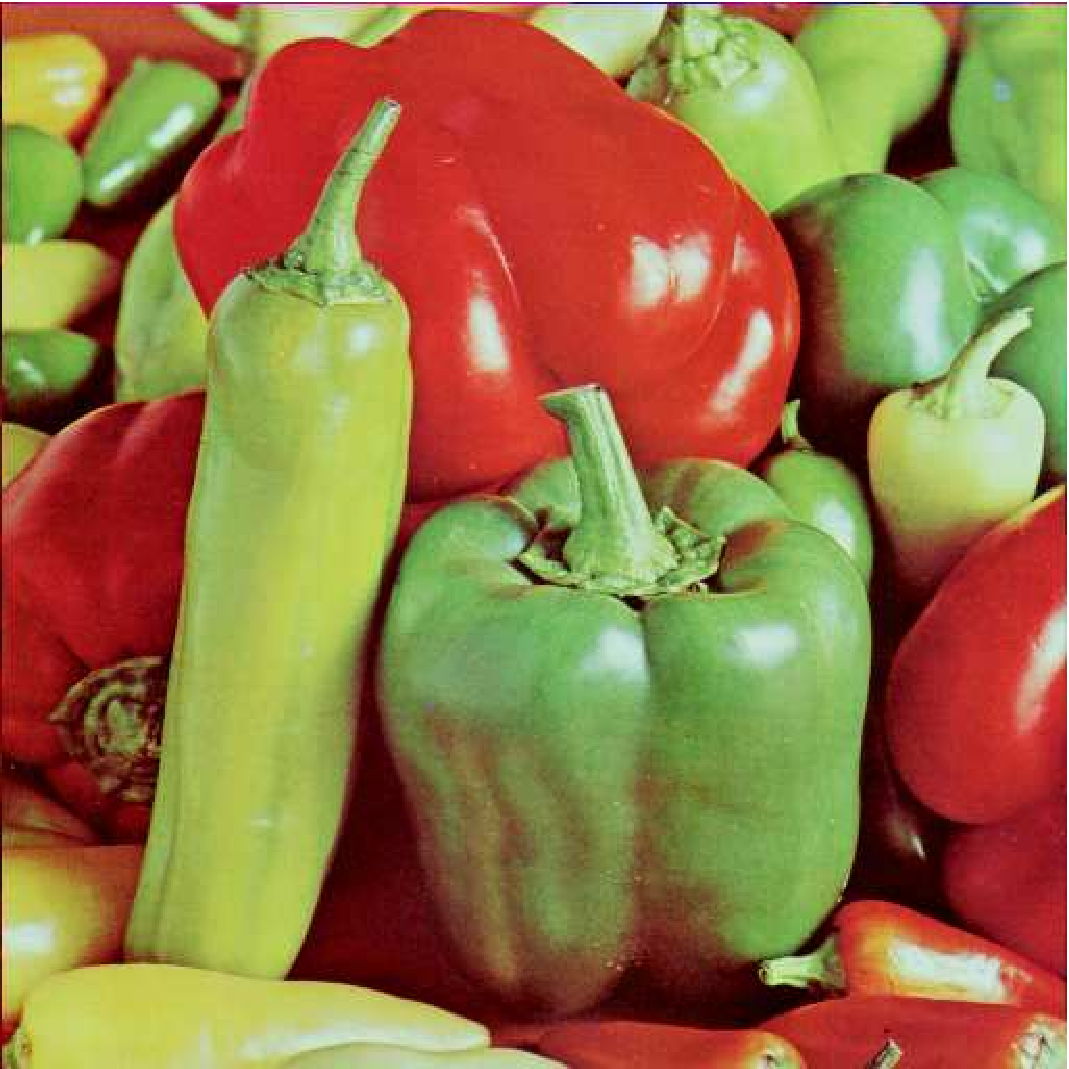
\includegraphics[width=0.95\textwidth]{images/peppers}
\end{minipage}%
\begin{minipage}[b]{0.25\textwidth}
RGB, R:\\
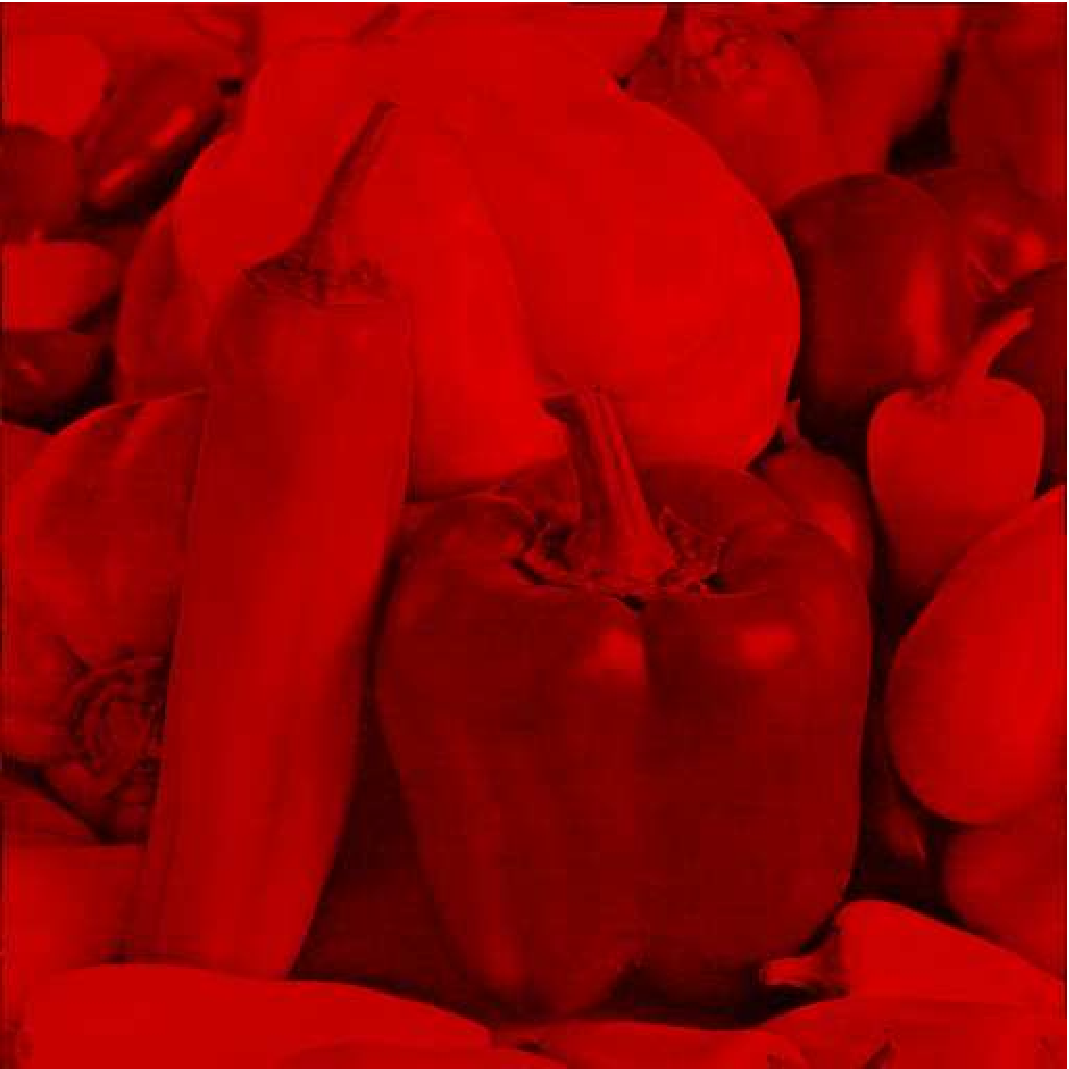
\includegraphics[width=0.95\textwidth]{images/rgbR}
\end{minipage}%
\begin{minipage}[b]{0.25\textwidth}
RGB, G:\\
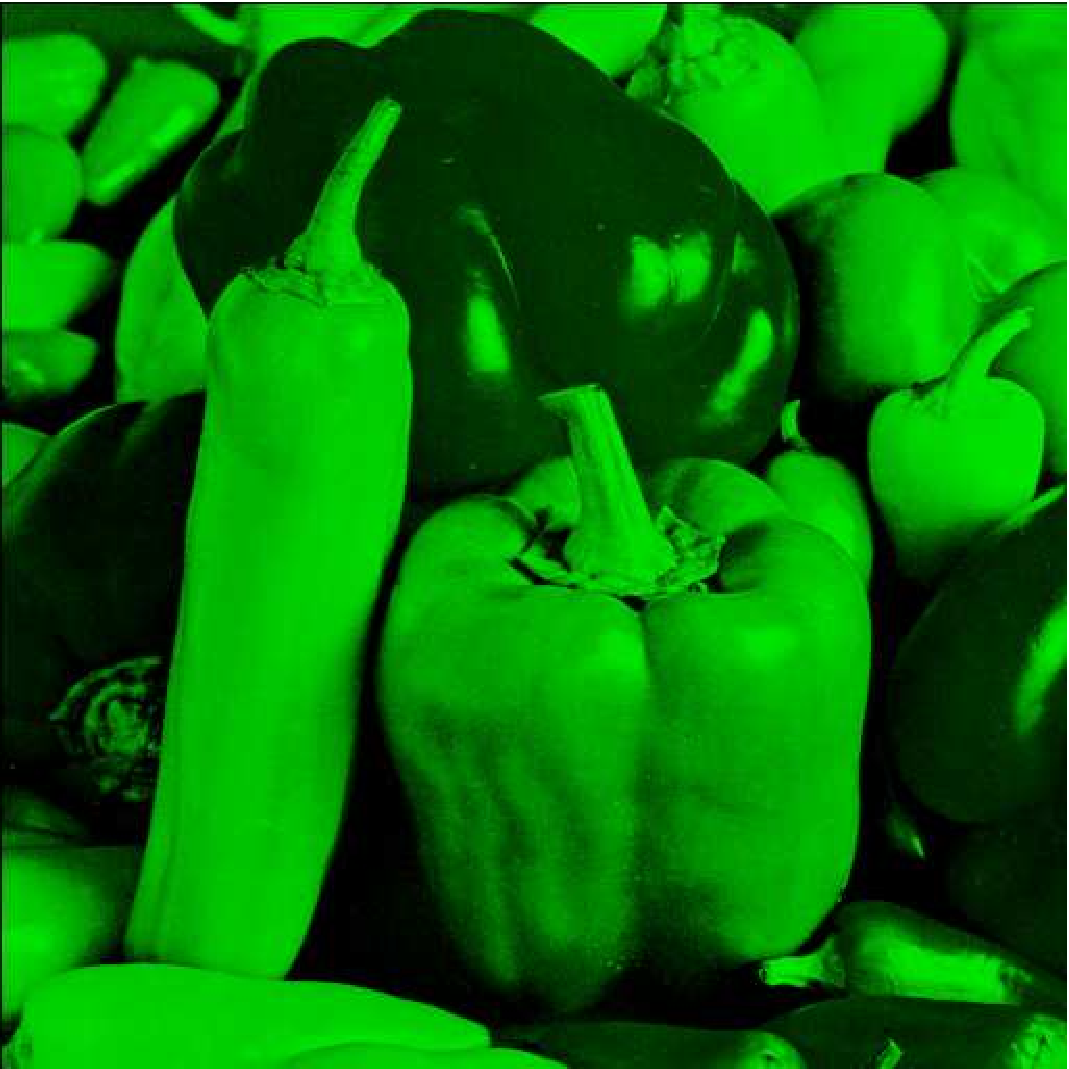
\includegraphics[width=0.95\textwidth]{images/rgbG}
\end{minipage}%
\begin{minipage}[b]{0.25\textwidth}
RGB, B:\\
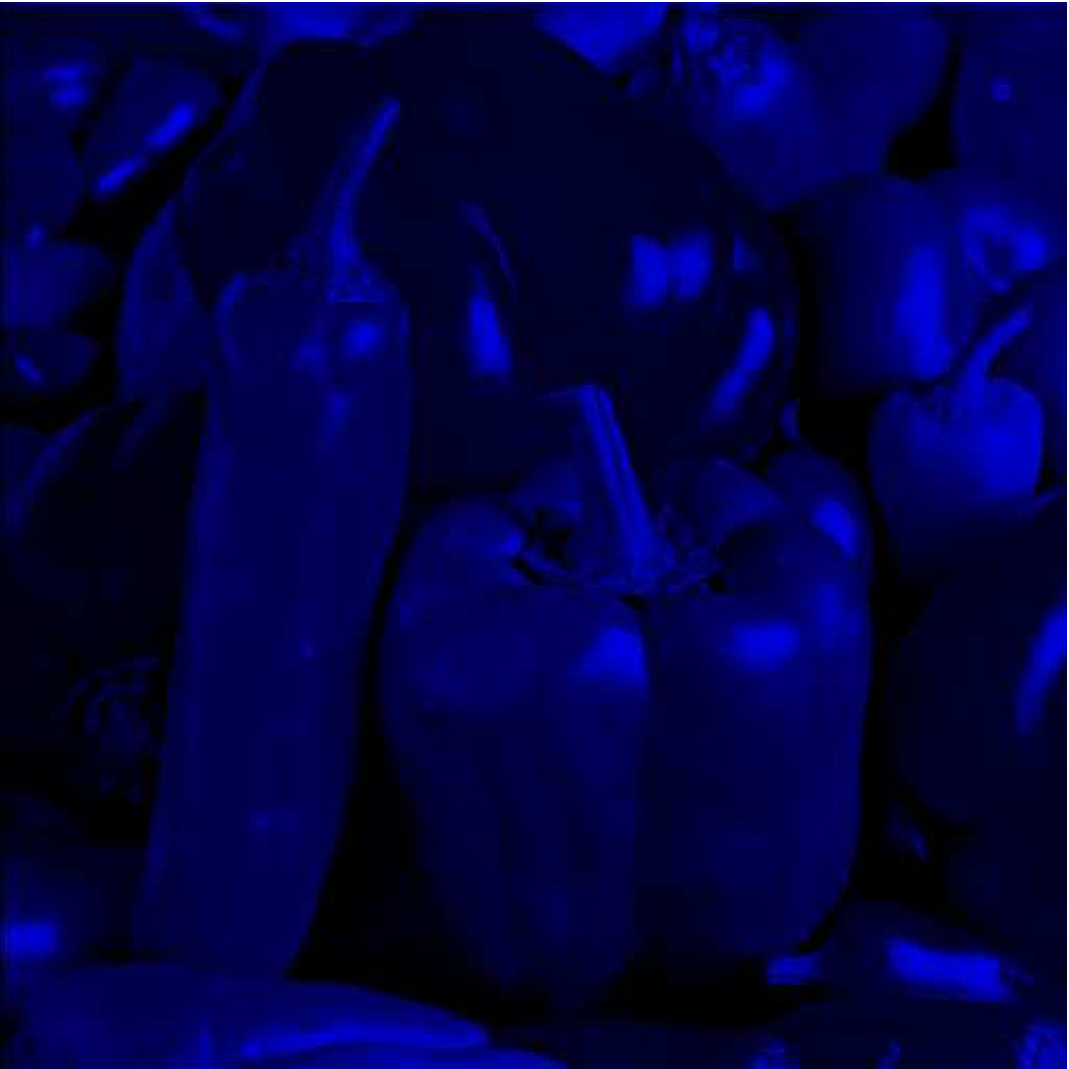
\includegraphics[width=0.95\textwidth]{images/rgbB}
\end{minipage}%

\medskip

\begin{minipage}[b]{0.33\textwidth}
YIQ, Y:\\
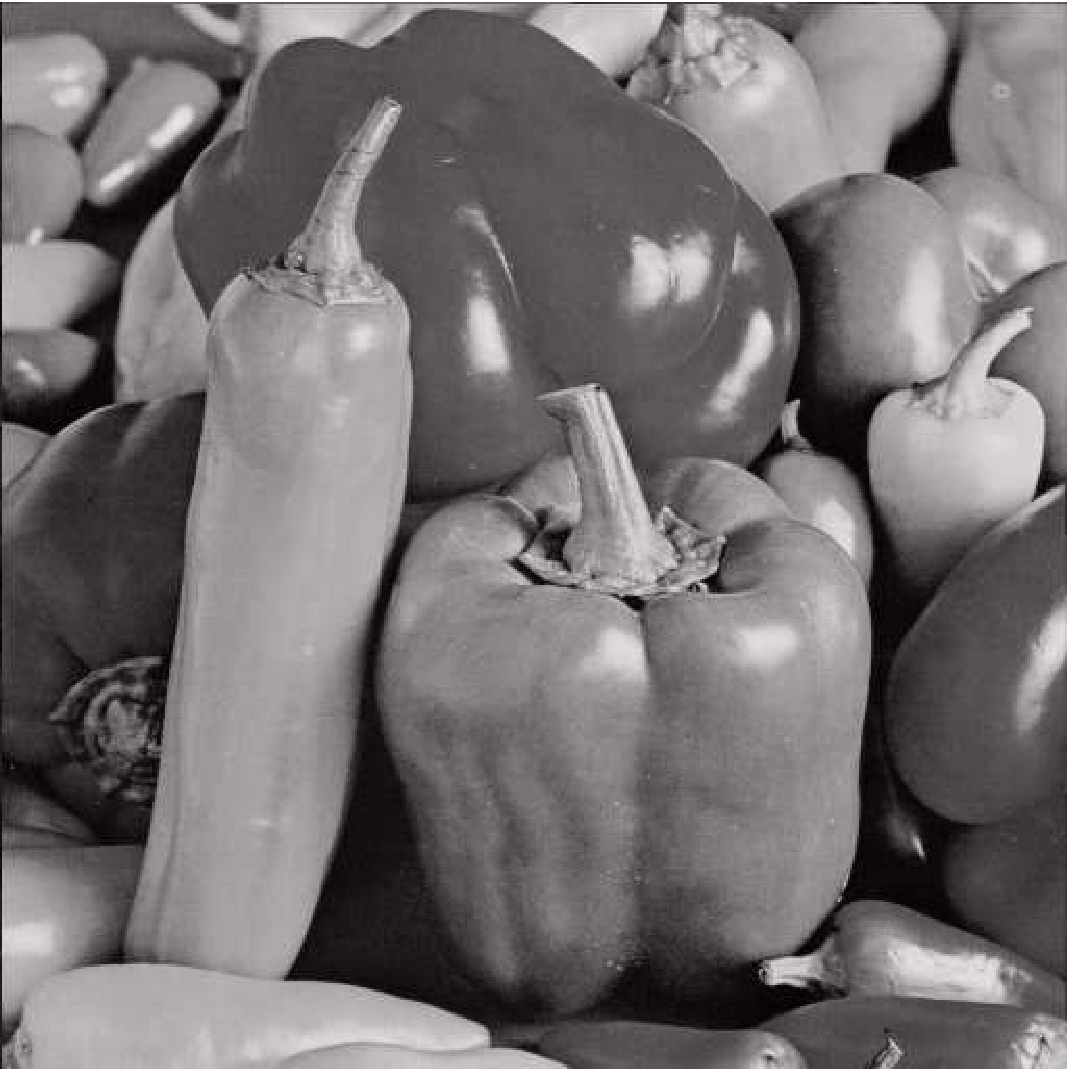
\includegraphics[width=0.95\textwidth]{images/yiqY}
\end{minipage}%
\begin{minipage}[b]{0.33\textwidth}
YIQ, I:\\
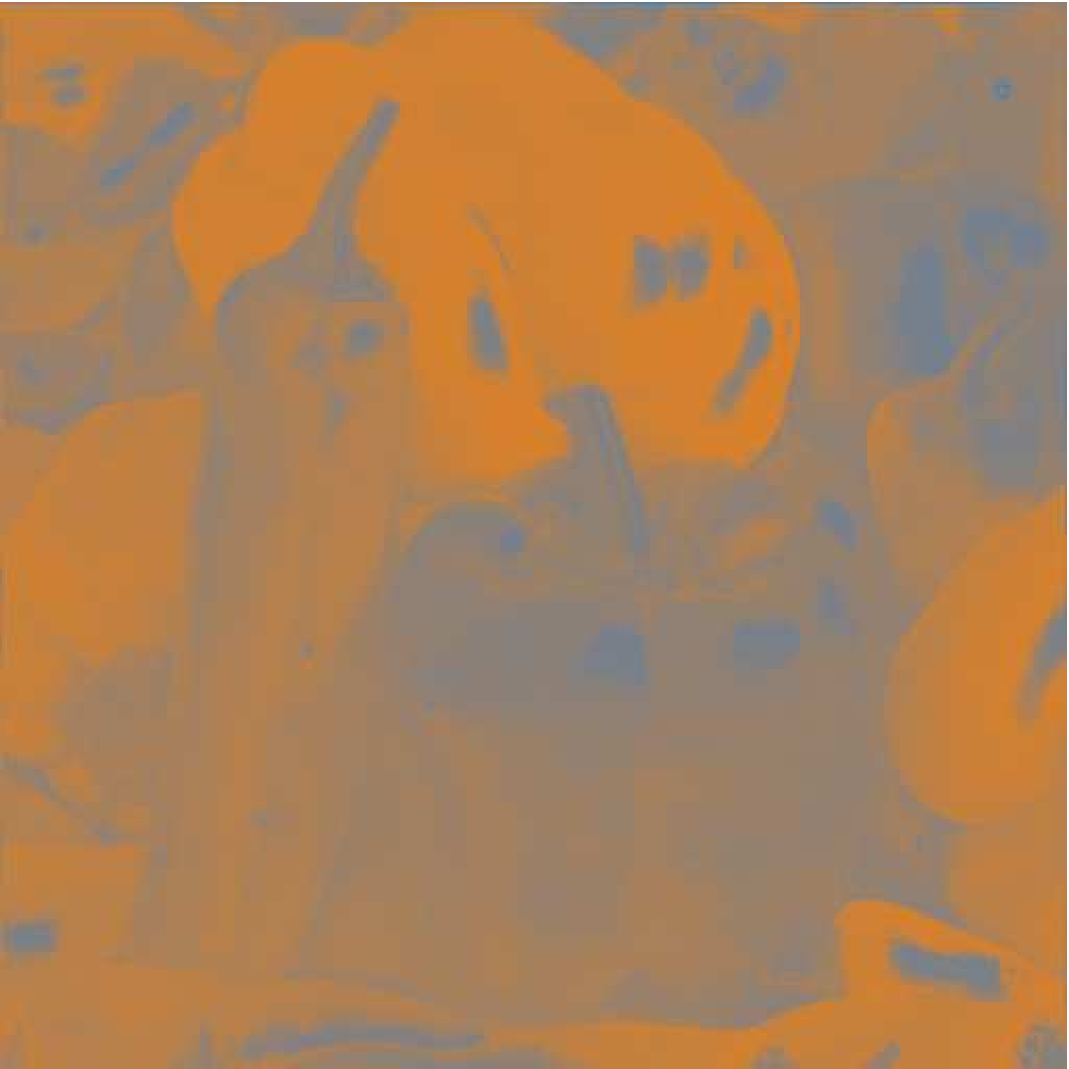
\includegraphics[width=0.95\textwidth]{images/yiqI2}
\end{minipage}%
\begin{minipage}[b]{0.33\textwidth}
YIQ, Q:\\
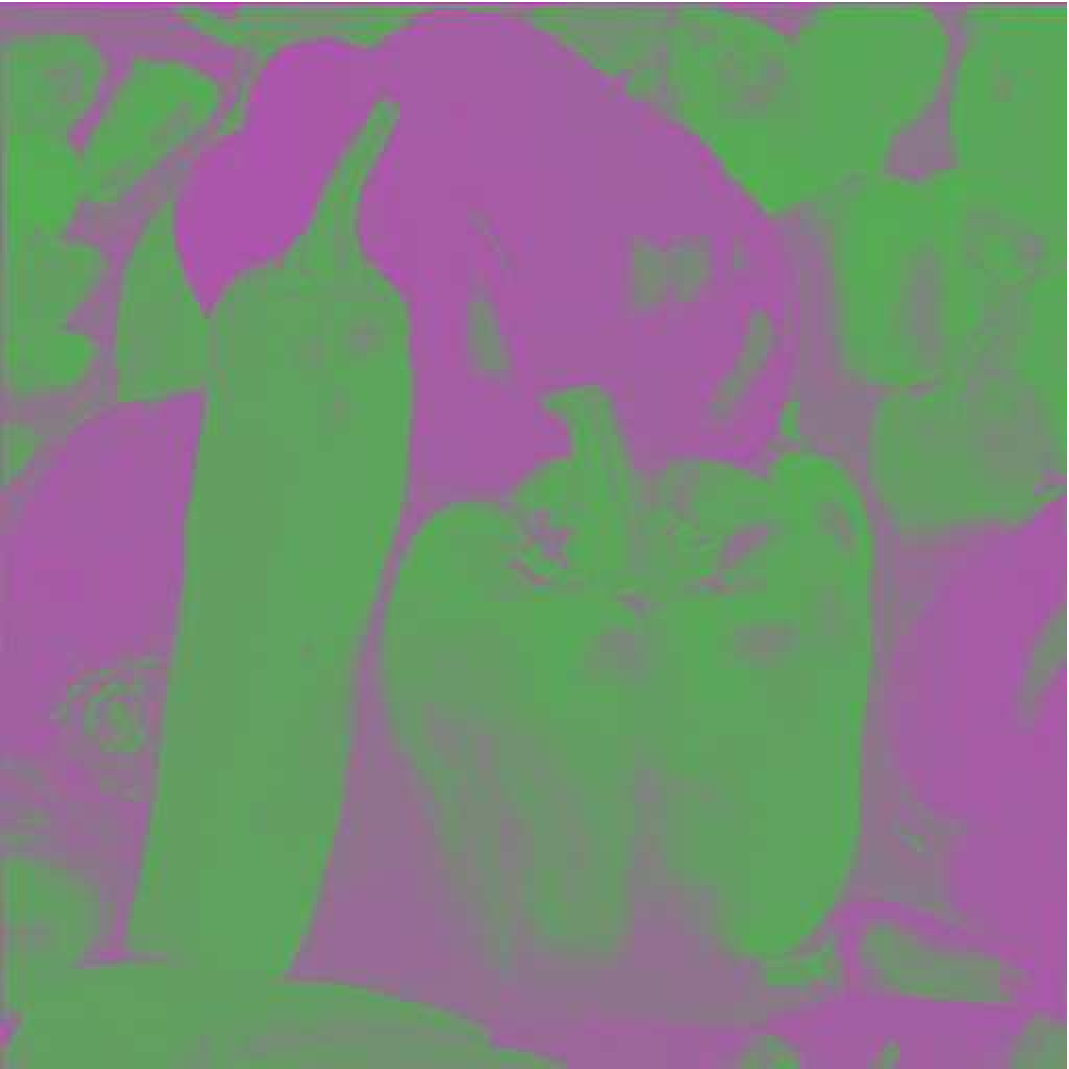
\includegraphics[width=0.95\textwidth]{images/yiqQ2}
\end{minipage}%

\medskip

\begin{minipage}[b]{0.33\textwidth}
YCbCr, Y:\\
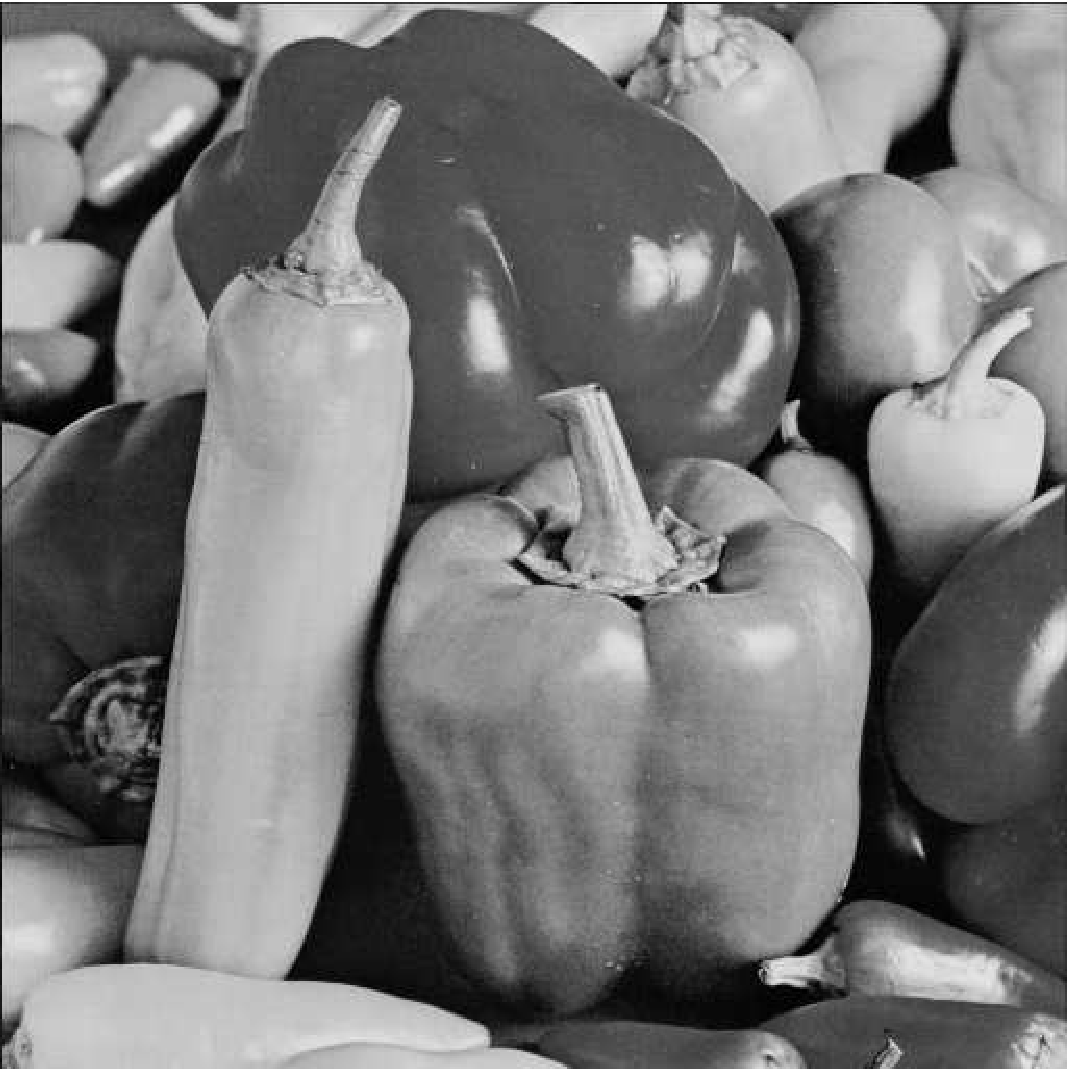
\includegraphics[width=0.95\textwidth]{images/ycbcrY}
\end{minipage}%
\begin{minipage}[b]{0.33\textwidth}
YCbCr, Cb:\\
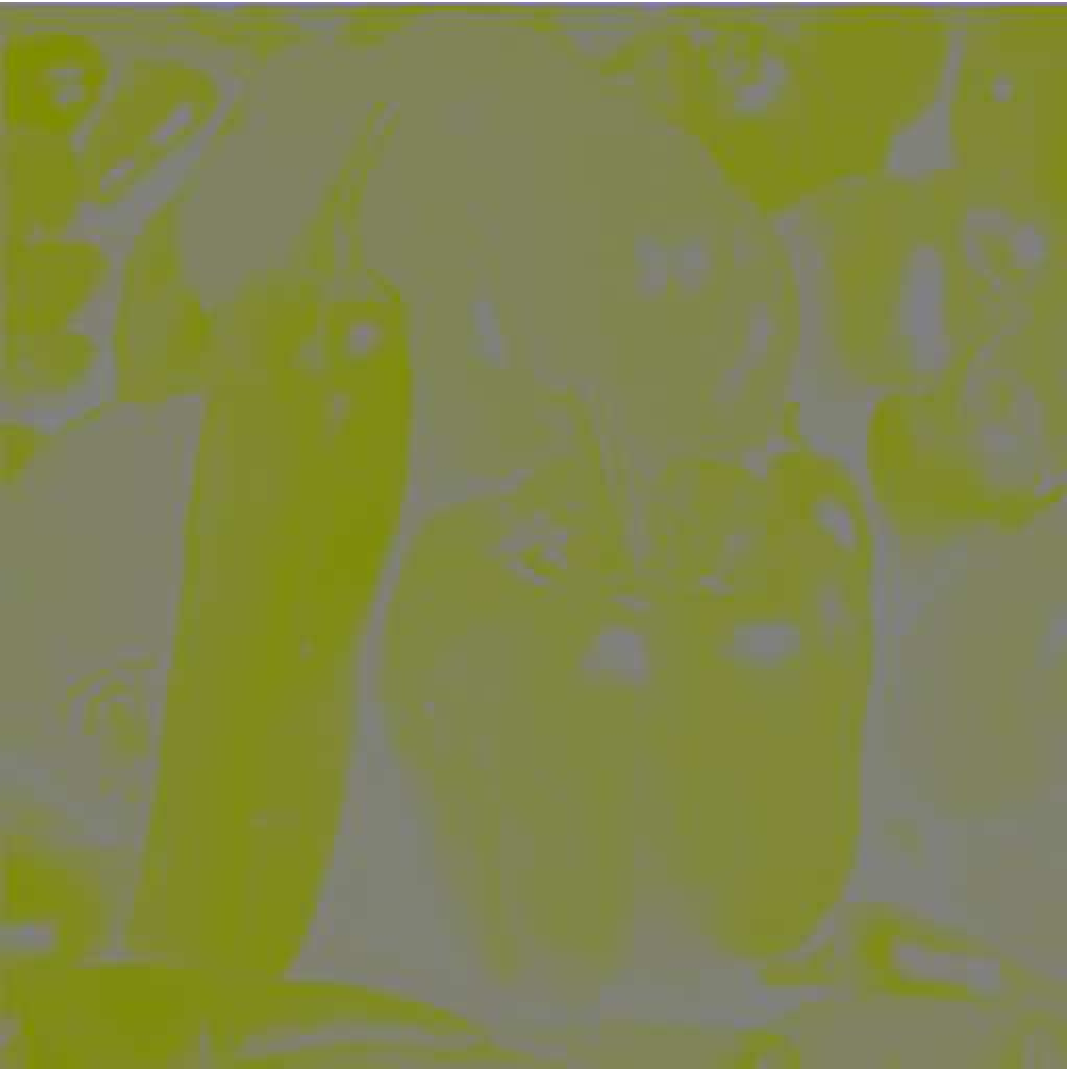
\includegraphics[width=0.95\textwidth]{images/ycbcrCr2}
\end{minipage}%
\begin{minipage}[b]{0.33\textwidth}
YCbCr, Cr:\\
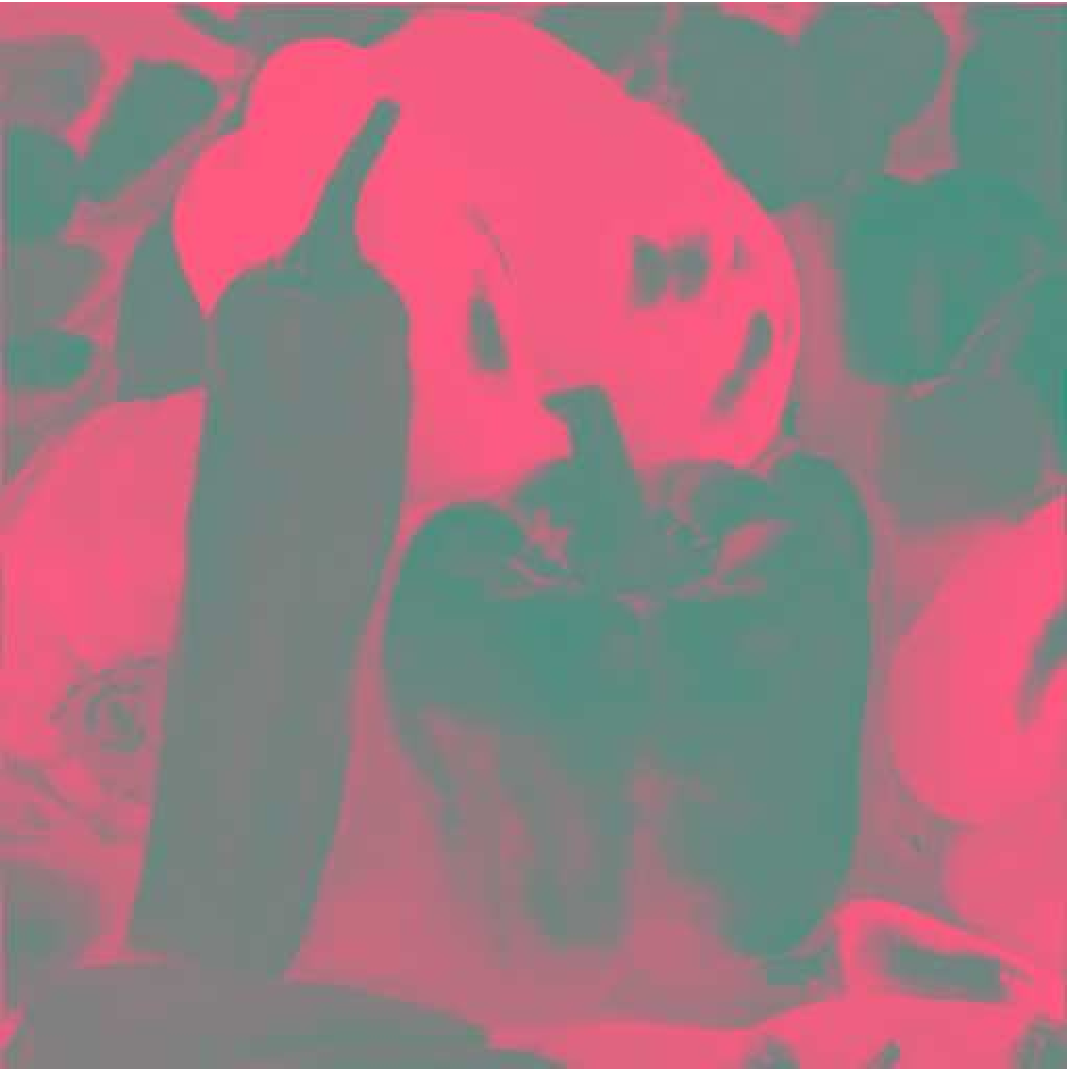
\includegraphics[width=0.95\textwidth]{images/ycbcrCb2}
\end{minipage}%

\caption{Three color decompositions: RGB, YCbCr, and YIQ.}
\label{fig:colorspaces}
\end{figure}

Figure~\ref{fig:colorspaces} shows three different color decompositions for the
same image: RGB (red, green, blue), YCbCr (luminance, blue-ness, red-ness),
and YIQ (luminance, orange-blue, purple-green).

In RGB, different shades of gray correspond to RGB triples where $R=G=B$,
e.g. black is (0,0,0) and white is ($2^b-1$,$2^b-1$,$2^b-1$) if $b$ is the bit depth.
The other two color spaces have one luminance channel (Y) and two ``chroma'' (color) channels.
Shades of gray correspond to different values for Y, while the chroma channels are zero.

\subsubsection{The YIQ Color Space}

Many compression algorithms, e.g. JPEG, use the YCbCr color space.
They typically use a non-reversible transformation from RGB to YCbCr, which is a (small) source
of information loss. In the YCbCr color space, both chroma channels are equally important.
In the YIQ color space however, the I channel is ``more important'' than the Q channel in the
sense that the human eye is more sensitive to slight variantions in I value than in variations
in Q value. In either color space, the Y channel is by far the most important one.


\begin{figure}
%GNUPLOT: LaTeX picture with Postscript
\begin{minipage}[b]{0.5\textwidth}
Cb-Cr plane:\\
\begin{picture}(0,0)%

\includegraphics[width=0.95\textwidth]{images/CbCr}%
\end{picture}%
\begingroup
\setlength{\unitlength}{0.00095\textwidth}%
\begin{picture}(1000,1000)(0,0)%
\put(500,100){\makebox(0,0)[c]{\strut{} max Cb}}%
\put(500,900){\makebox(0,0)[c]{\strut{} min Cb}}%
\put(0,500){\makebox(0,0)[l]{\strut{} min Cr}}%
\put(1000,500){\makebox(0,0)[r]{\strut{} max Cr }}%
\end{picture}%
\endgroup
\end{minipage}%
\begin{minipage}[b]{0.5\textwidth}
I-Q plane:\\
\begin{picture}(0,0)%

\includegraphics[width=0.95\textwidth]{images/IQ}%
\end{picture}%
\begingroup
\setlength{\unitlength}{0.00095\textwidth}%
\begin{picture}(1000,1000)(0,0)%
\put(500,100){\makebox(0,0)[c]{\strut{} max I}}%
\put(500,900){\makebox(0,0)[c]{\strut{} min I}}%
\put(0,500){\makebox(0,0)[l]{\strut{} min Q}}%
\put(1000,500){\makebox(0,0)[r]{\strut{} max Q }}%
\end{picture}%
\endgroup
\end{minipage}%
\caption{The Cb-Cr and I-Q color planes.}
\label{fig:cbcr-iq}
\end{figure}


We will use an approximation of the YIQ color space.
The Y channel is most important, and will get priority over both the chroma channels.
The I channel is somewhat more important than the Q channel. If an alpha channel is present,
it is considered even more important than the Y channel.




\subsubsection{Reversible Transformation}

Figure~\ref{fig:cbcr-iq} shows the difference between the Cb-Cr plane and the
(approximated) I-Q plane. It shows the planes at an intermediate value for Y.
The accurate transformation from RGB to YIQ is as follows:
$$
\left(
\begin{array}{c}
y \\ i \\ q
\end{array}
\right)
=
\left(
\begin{array}{ccc}
0.299  & 0.587   & 0.114 \\
1.0    & -0.4607 & -0.5393 \\
0.4046 & -1.0    & 0.5954
\end{array}
\right)
\left(
\begin{array}{c}
r \\ g \\ b
\end{array}
\right)
$$

When converting from RGB to YIQ using floating point arithmetic with the above formula,
rounding errors will make sure that the reverse transformation from YIQ to RGB will not
always result in the original RGB values.
To be able to do lossless compression, we need a reversible transformation.
We use the following reversible integer arithmetic approximation\footnote{We did not come up with this reversible YIQ transform. It was described
in a paper, but I can't find the reference anymore. If you know the paper I'm talking about, please let me know!}:
$$
\left\{
\begin{array}{ccl}
y & = & ((r+b)/2 + g)/2\\
i & = & r-b \\
q & = & (r+b)/2 - g\\
\end{array}
\right.
$$
where the divisions are integer divisions.
This more or less corresponds to the following transformation matrix:
$$
\left(
\begin{array}{ccc}
0.25  & 0.5   & 0.25 \\
1.0   & 0     & -1.0 \\
0.5   & -1.0  & 0.5 \\
\end{array}
\right)
$$
The approximation is quite rough (especially for $i$), but it will do.
Note that we convert three $k$ bit numbers to one $k$ bit number and two $k+1$ bit numbers:
the $i$ and $q$ have a larger range. Instead of using a sign bit, we add $2^k-1$ to $i$ and $q$
so they are in the range $[0..2^{k+1}-2]$.

% TODO : find reference to the reversible transformation


\subsection{Auto-Indexing}
\label{sec:auto-indexing}

Many images only use a small fragment of the full color space. We can avoid redundancy
if we can take that into account. For example, if the image is actually a grayscale image,
the values for I and Q are always zero.

We record the minimum and maximum value that occurs for each channel (Y, I, and Q), so every number that
is outputted will be in that range. The smaller the range, the lesser the number of bits
needed to output a number in the range. For a singleton range no bits are needed at all.

These global ranges only give a rough indication of the colors that occur: they only describe
a bounding box in the three-dimensional color space.
Photographic images typically use large continuous ranges of colors, but line drawings
and other non-photographic images often use only a relatively small number of discrete colors.
Image formats like GIF and PNG use an index of colors (called the {\it palette}; typically no more
than 256 different colors can be used) to encode such images concisely.
If the total number of colors is low enough, it is a good idea to use a palette.
FLIF can work with arbitrary palette sizes; the default maximum palette size is 512.

If the image has a nontrivial alpha channel (i.e. it is not fully opaque), then FLIF will attempt
to make a palette consisting of YIQA colors. If there are too many different colors, then FLIF
will attempt to make a palette consisting of YIQ colors, encoding the alpha channel separately.

However, the palette approach only covers images which use a very small fragment of the full color space.
Some images contain a mix of continuous color ranges and discrete colors. For example, an
image that contains a rendering of a document that contains both (anti-aliased) text and
diagrams (e.g. generated by gnuplot)
will typically use the entire grayscale range (256 colors) and a small number of non-gray colors.
If the colored lines are also anti-aliased, then the total number of colors can quickly grow too
big to be represented effectively using an indexed palette, but the image still only uses a relatively small
fragment of the full color space.

We propose a simple yet effective mechanism, called {\it auto color buckets} (ACB),
that generalizes the idea of color palettes. It works as follows.

For each value of Y, we keep track of the I values that occur for that value. As long as the number of
distinct I values for a given Y value is small, we maintain a list of discrete values (a ``discrete bucket'');
if that list becomes too large (according to some rather arbitrary threshold),
then we replace it by an interval, storing only the lower and upper bounds (a ``continuous bucket'').
Then for each combination of Y and I, we keep track of the Q values that occur, in a similar way.
To keep the total number of buckets reasonable, quantization can be used.


Using this method, we get an approximate ``color profile'' of the image.
We will later make use of this profile in order to avoid writing redundant bits when outputting pixels.


\subsubsection{Color Bucket Simplification}

Obviously the decoder cannot compute the color profile from the original image, so the
color information has to be outputted during encoding so the decoder can load the information.


Even when compressed, outputting the color table can be quite costly in terms of space (several kilobytes),
and it may not always be worth it. We use a heuristic to decide when to output the color table
and when to skip it.

Photographic images typically use a rather large fragment of the total color space,
and the color table will usually consist of a number of continuous buckets and a number
of discrete buckets which contain a large amount of colors (close to the threshold).
These discrete colors are usually not far removed from one another.

The size of the color table can be reduced by converting discrete buckets to continuous
buckets. We do this if the discrete bucket has at least 3 different colors and the volume of the
bounding box of those colors is not much bigger than the size of the list.



\section{Image Traversal}
\label{sec:traversal}

We have implemented two different methods to traverse the image.
The first method is a very simple scanline traversal; it is discussed in Section~\ref{sec:simple_traversal}.
This method somewhat faster and easier to implement than the second one, but it is not suitable for progressive decoding.
The second method is a generalization of PNG's Adam7 interlacing --- it could be called ``Adam$\infty$ interlacing''.
It is somewhat more complicated and slower, but it is suitable for progressive decoding.
This second method, which is FLIF's default method, will be discussed in Section~\ref{sec:interlacing}.

\subsection{Simple Scanline Traversal}
\label{sec:simple_traversal}

The first traversal method is similar to the one used in many other image compression formats, including
non-interlaced PNG, non-interlaced GIF, WebP and FFV1.

The image is scanned line by line from top to bottom. Each line is scanned from left to right.
When outputting a pixel, the value of the neighboring pixels above and to the left are already outputted,
so those values can be used to compute a prediction that is also available at decode time.

\subsubsection{Pixel prediction}
Assume the pixel to be outputted is $X$:
\begin{center}
\begin{tabular}{|c|c|}
\hline
$A$ & $B$ \\
\hline
$C$ & $X$ \\
\hline
\end{tabular}
\end{center}
As a prediction for $X$ (the pixel to ``guess''), we take the median of the following three values:
$B$ (top), $C$ (left), and $B+C-A$ (gradient). This guess will be correct if the local area
of the image happens to contain a smooth linear color gradient. This predictor is exactly the same as the one
used in the FFV1 lossless video codec.

We compute the guesses separately for each channel in the YIQ color space.
Then we compute the difference between the guessed values and the actual values,
and we output those. If the guess was good, those differences will be zero or close to zero.

Note that the differences can be positive or negative. At first sight, their range
is twice as large as the range of the original numbers. However, given the guess, only
half of that range is valid. We also take into account that not all YIQ triples correspond
to valid RGB triples, and if available, the color profile of the image (see Section~\ref{sec:auto-indexing})
can further reduce the number of possible values for the difference. The color profile (if available)
is also be used to ``snap'' the guessed value to a value that is valid w.r.t. the relevant color bucket:
if the color bucket is discrete, the guess gets ``rounded'' to the nearest value in the list;
if the color bucket is continuous, then the guess gets clipped to the interval.
This will be discussed in more detail in
Sections \ref{sec:rac:interval} and \ref{sec:rac:bitvector}.



\subsection{Adam$\infty$ Interlacing}
\label{sec:interlacing}

The aim of interlacing is to be able to progressively reconstruct a compressed image, perhaps even
not loading the entire compressed stream if it is a large image and only a small preview is needed.
FLIF uses a generalization of PNG's Adam7 interlacing. In each interlacing step, the number of pixels
roughly doubles (exactly if the image is a square $2^n$ by $2^n$ image) 

The first pixel outputted is the pixel in the left-top corner of the image. Counting rows and columns from zero
and from top to bottom, left to right, this is the pixel at position $(0,0)$.
Then, in each interlacing step, either the number of rows doubles (a horizontal step),
or the number of columns doubles (a vertical step). The final step is always a horizontal step, traversing all the
odd-numbered rows of the image.

\subsubsection{Pixel prediction}
\label{sec:prediction_interlacing}

There are two cases, which are similar up to rotation.
In the case of a horizontal step, we have the following situation in general:

\begin{center}
\begin{tabular}{|c|c|c|c|c|}
\hline
$A$ & $B$ & $C$ \\
\hline
$P$ & $X$ &  \\
\hline
$D$ & $E$ & $F$ \\
\hline
\end{tabular}
\end{center}

where $A$, $B$, $C$, $D$, $E$ and $F$ are known pixels (from a previous interlacing step), $P$ is also known
(it is the pixel previously outputted in the current interlacing step), and $X$ is
the pixel to be outputted.

We use as a prediction for $X$ the median of these three values:
\begin{itemize}
\item the linear interpolation between top and bottom: $(B+E)/2$
\item the top-left gradient $P+B-A$
\item the bottom-left gradient $P+E-D$
\end{itemize}
The top-left gradient is also used in the scanline traversal method, but the other two values are based on pixels $D$ and $E$ which
would not be known during decoding in the scanline traversal method.

In the case of a vertical step, we have the following situation in general:

\begin{center}
\begin{tabular}{|c|c|c|c|c|}
\hline
$A$ & $P$ & $D$ \\
\hline
$B$ & $X$ & $E$ \\
\hline
$C$ &     & $F$ \\
\hline
\end{tabular}
\end{center}

where $A$, $B$, $C$, $D$, $E$ and $F$ are known pixels (from a previous interlacing step), $P$ is also known
(it is a pixel outputted in the current interlacing step), and $X$ is
the pixel to be outputted.

We use as a prediction for $X$ the median of these three values:
\begin{itemize}
\item the linear interpolation between left and right: $(B+E)/2$
\item the top-left gradient $P+B-A$
\item the top-right gradient $P+E-D$
\end{itemize}


The gradients can have a value which is outside the valid range:
e.g. if the range is $[0,255]$ then the gradient can get a value as large as $510$ and as low as $-255$.
In the case of scanline traversal, this is not an issue because we take a median of two actual pixel values and
one gradient, so the median will always be inside the valid range. This is no longer the case with this predicted value:
e.g. with $B=E=P=255$ and $A=D=0$ we would take the median of $255$, $510$ and $510$, which is $510$.
To keep the predicted value sane, we therefore snap it to the valid range --- taking into account the global bounds
and the color buckets, if available.

\subsection{Channel Ordering}
So far, we have only considered a single channel of pixel values, i.e. a grayscale image.
When using scanline traversal, we simply process all the channels. We first output the alpha channel (if there is one),
then the Y channel, then the I channel, and finally the Q channel.
If the value of a pixel in the alpha channel is equal to zero, then this pixel is completely transparent. This means that
its values in the other channels are irrelevant.\footnote{At least, that is our opinion. One can also argue that the alpha channel
can be used to mask parts of an image but the original image ``behind the mask'' should be kept intact, even when pixels are completely masked.}
For this reason, the alpha channel is outputted first, so the other channels are only encoded where the alpha value is nonzero.

Still, those ``irrelevant'' pixels need to get Y, I and Q values, because they can be referred to when predicting ``relevant'' pixels.
(Also, as a more practical consideration, the output formats to decompress to --- PNG and PAM --- expect all pixels to have values for all channels.)
In the case of scanline traversal, we replace the Y,I,Q values of $A=0$ pixels by their prediction. This is well defined even though
that prediction itself may refer to earlier $A=0$ pixels.
For interlaced traversal, we replace the Y,I,Q values of $A=0$ pixels by the linear interpolation between the adjacent pixels (top-down or left-right)
from the previous interlace step.

When using interlaced traversal, the different channels are interleaved in such a way that the alpha channel and the Y channel
get encoded earlier at higher resolutions than the chroma channels.


\section{Entropy Encoding: MANIAC}
\label{sec:rac}

We use context-adaptive binary arithmetic coding (CABAC), based on the ideas of
the FFV1 codec \cite{FFV1}.
Arithmetic coding \cite{ArithmeticCoding}, also known as range encoding,
is a form of entropy encoding based on a probability model for the outputted symbols.


\subsection{CABAC mechanism}

In CABAC, the symbols are bits and the probability model is adaptive.
Since we are working with bits, the probability distribution can be expressed with
a single number, e.g. the chance to output 1. Initially we start with some arbitrary
chance (e.g. 50\%).
After outputting a bit, the chance is updated. The idea is to ``learn'' the actual
distribution from the observed past outputs in order to be able to have better predictions
for the future outputs. The same chance updates can be done when decoding since the update is
only based on previously outputted bits.

The above describes adaptive binary arithmetic coding. If we have additional ``context''
information about the outputted bits, we can use a different probability for each context.
If there is a correlation between the context information and the distribution of the
actual symbols, this can lead to more accurate probability estimates and hence better compression.
Obviously the context information also needs to be available at decode time.




\subsubsection{Integer Encoding Given Interval}
\label{sec:rac:interval}

In the FLIF algorithm (and also in FFV1) we need to output signed integers.
Of course integers can be represented in a binary representation, with a different chance
for every bit position, but the exponent-mantissa representation used in FFV1 turns out
to be better.

Suppose we want to output a value $x \in [-a,a]$.
First we output a single bit to indicate whether $x = 0$ or $x \neq 0$.
Then we output the sign of $x$, followed by the exponent, i.e. the number of bits $e = \lceil \log(|x|) \rceil$ needed to
represent $x$, where $e \in [1,\log(|a|)]$.
The number $e$ is outputted in {\em unary} as $e$ 1 bits followed by one 0 bit.
We use different chances for each of these exponent bits.
Finally we output the mantissa bits; the leading 1 can be omitted since we already know the exponent.




In general, if we know the value to be outputted $x$ is in the interval $[a,b]$, some of the
above output bits are redundant. If the interval does not contain zero, the zero-bit does not
need to be outputted. If the signs of $a$ and $b$ are the same, the sign-bit does not need to be
outputted. In some cases we have a lower bound on the exponent, e.g. if $x \in [32,80]$ then
we know $e \geq 5$ so the first 5 exponent bits can be omitted. If the exponent has the largest
possible value (e.g. 6 if $x \in [32,80]$), then it does not need to be followed by a 0 bit.
Finally, when outputting the mantissa, some bit values may be impossible, e.g. if $x \in [32,80]$ and
$e=6$ (so $x \in [64,80]$), then the most significant outputted bit of the mantissa
(the one for 32) cannot be 1 since that would give a lower bound $x \geq 92$.
If one of the two bit values is impossible, it is implied that the bit must have the other value
so it does not need to be outputted.





\subsubsection{Multiscale CABAC}
\label{sec:multiscale}

As discussed before, after outputting a bit, the chance is updated in such a way that
the outputted value becomes more likely. We can choose the amount by which
the chance is increased or decreased. If the bits to be outputted are very predictable
(e.g. a long series of zeroes followed by a long series of ones),
it is a good idea to make large changes so repeated bits become cheap quickly.
However, if the outputted bits are less predictable (e.g. a random sequence where 0 has a probability
of 0.3 and 1 has a probability of 0.7), small changes are more suitable because
they allow convergence to the optimal value instead of constantly ``overshooting'' the target.

In order to get the best of both worlds, we use a {\em multiscale} chance model.
Instead of storing one chance with a fixed update speed
(a compromise between ``too fast'' and ``too slow''),
we store several chances and update them in different ways.
This allows us to consider different ``scales'': one to capture short-term fluctuations,
one to model the medium-term behavior, one long-term scale that changes only very slowly, etc.
For each scale, we store not only the current chance, but also the total number of bytes
(of compressed output)
that would have been outputted if that scale had been used.
We only actually use the scale that is currently the best one, i.e. the one that lead to the best
compression so far.





\subsection{Contexts}

In FFV1, quantized sample differences are used as context information.
If the current pixel is $X$, then the following known neighbor pixels are used to compute the
context:
\begin{center}
\begin{tabular}{|c|c|c|c|}
\hline
  & & $TT$ & \\
\hline
  & $TL$ & $T$ & $TR$ \\
\hline
$LL$ & $L$ & $X$ & \\
\hline
\end{tabular}
\end{center}

The five differences $L-TL$, $TL-T$, $T-TR$, $LL-L$, $TT-T$ are computed and quantized (using
a logarithmic scale).
For every combination, a different context is defined.
In total, 7563 different contexts (per color channel) are used in the ``large'' context model of FFV1.


\subsubsection{Relevant Pixel Properties}

The contexts depend on the image traversal order (see Section~\ref{sec:traversal}).

\paragraph{Scanline traversal.}
In this mode, we use the same five differences as in the ``large'' context model of FFV1 (but without quantization),
and we also use the following extra properties:
\begin{description}
\item[Other channels]: The value of the pixel in all of the other channels that are already known (at most three: A, Y, and I)
\item[Median-index]: The pixel prediction computes a median of 3 values. This property has the value $0$, $1$ or $2$ and encodes which of those 3 values was used.
\item[Prediction]: The predicted value itself
\end{description}
In total, for pixels in the alpha channel, there are 7 properties, for pixels in the Y channel there are 7 or 8 properties
(depending on whether there is an alpha channel), for pixels in the I channel there are 8 or 9 properties, and for pixels
in the Q channel there are 9 or 10 properties.


\paragraph{Interlaced traversal.}
The above two to five properties are also used in the interlacing mode. The five properties from the
``large'' context model of FFV1 are also used for the alpha and Y channels; for the I and Q channels,
$LL-L$ and $TT-T$ are omitted. Additionally, one more property is used, depending on the direction of the interlacing step:
\begin{description}
\item[Horizontal step]: top - bottom
\item[Vertical step]: left - right
\end{description}
Referring to section~\ref{sec:prediction_interlacing}, in both cases this corresponds to $B-E$.

In total, for pixels in the alpha channel, there are 8 properties, for pixels in the Y channel there are 8 or 9 properties
(depending on whether there is an alpha channel), for pixels in the I channel there are 7 or 8 properties, and for pixels
in the Q channel there are 8 or 9 properties.

Since the space and time complexity of encoding (and, to a lesser extent, decoding) is proportional to the number of properties,
it makes sense to restrict the number of properties. This set of properties is more or less arbitrarily chosen.



\subsection{Context Tree Learning}
\label{sec:context_tree}

When using static contexts like in FFV1, where the number of contexts is the product of
domain sizes of each property, quantization has to be used in order to reduce
the number of contexts. It is hard to get the number of contexts ``just right''.
On the one hand, if you use too many contexts, it takes a lot of memory and it also reduces
the amount of probability model adaptation that can be done since the number of outputted
pixels per context is small. On the other hand, if you use too few contexts, compression also
suffers since pixels with different properties end up getting outputted in the same context.
Also, when the contexts are defined statically,
a lot of the contexts are actually not used at all since the corresponding
combination of properties simply does not occur in the source image.


By contrast, we propose a dynamic data structure to store the contexts. It is essentially
a decision tree (actually one tree per YIQA channel), which is grown from a single node.
Figure~\ref{fig:context_tree} shows an example of a ``context tree''.


\begin{figure}
\begin{center}
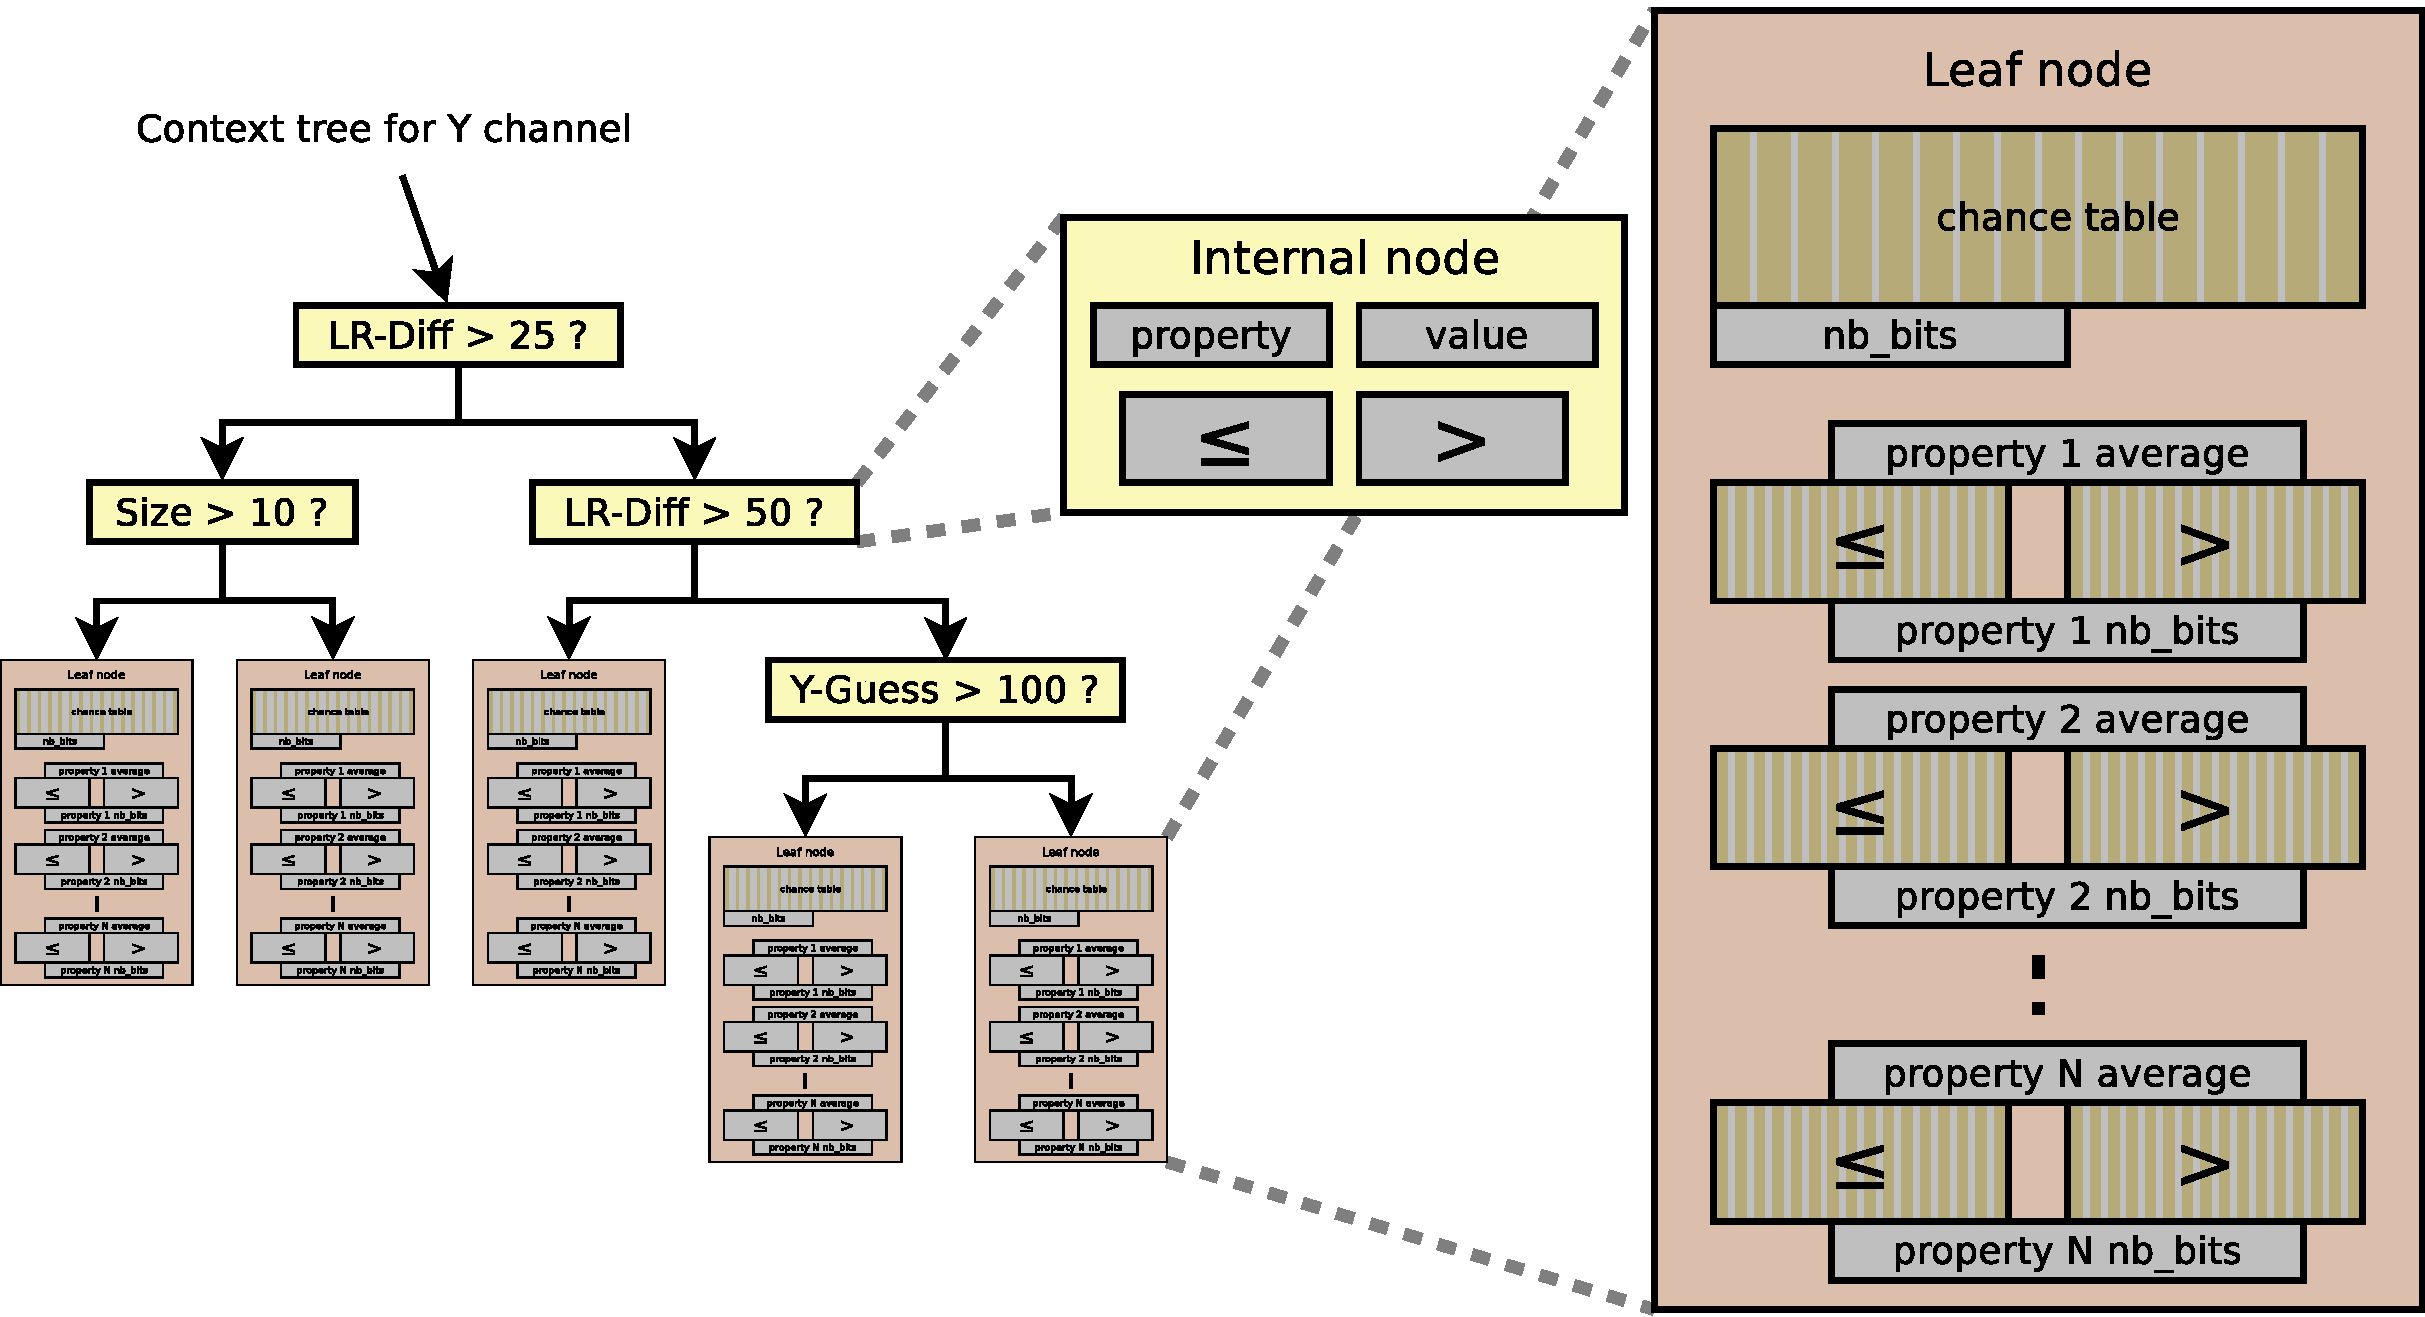
\includegraphics[width=\textwidth]{images/context_tree}
\end{center}
\caption{Context tree structure.}
\label{fig:context_tree}
\end{figure}

In every internal (non-leaf) node, there is a ``test'': an inequality comparing one of the properties
to some value. Every leaf node contains one ``actual'' context (array of chances)
and two ``virtual'' contexts per property, so at most 23 contexts in total.

When outputting a pixel, the decision tree is traversed until a leaf node is reached.
The actual context is used to output the value, and the number of bits needed to
represent the compressed output is added to a counter.
For each of the properties, we maintain a running average of its value within the leaf;
one virtual context is used for values below the average, the other is used for higher-than-average 
values. For each property we select the virtual context accordingly,
and we output the same output value again, but only ``virtually'', that is,
nothing is written to the compressed file, but the chances are updated and the bit counter
for that property is incremented.

The aim of the bit counters is to find out which property is most significant.
If a property is irrelevant, then the sum of the bit counts for its two virtual contexts will be the same
or higher than that of the actual context. If however a property is relevant, then using two different
contexts depending on the value for that property will result in better compression.
We compare the bit count of the ``best'' virtual contexts in a given leaf node with the
bit count of the actual context.
If the best virtual contexts are performing better than the actual context,
we use the virtual contexts instead of the actual context for output, maintaining
the actual context as if it was virtual.
When the difference between the best virtual context and the actual context
becomes larger than some fixed
threshold, the leaf node is converted to a decision node which tests the ``best'' property.
Figure~\ref{fig:context_tree_split} illustrates how this is done.


\begin{figure}
\begin{center}
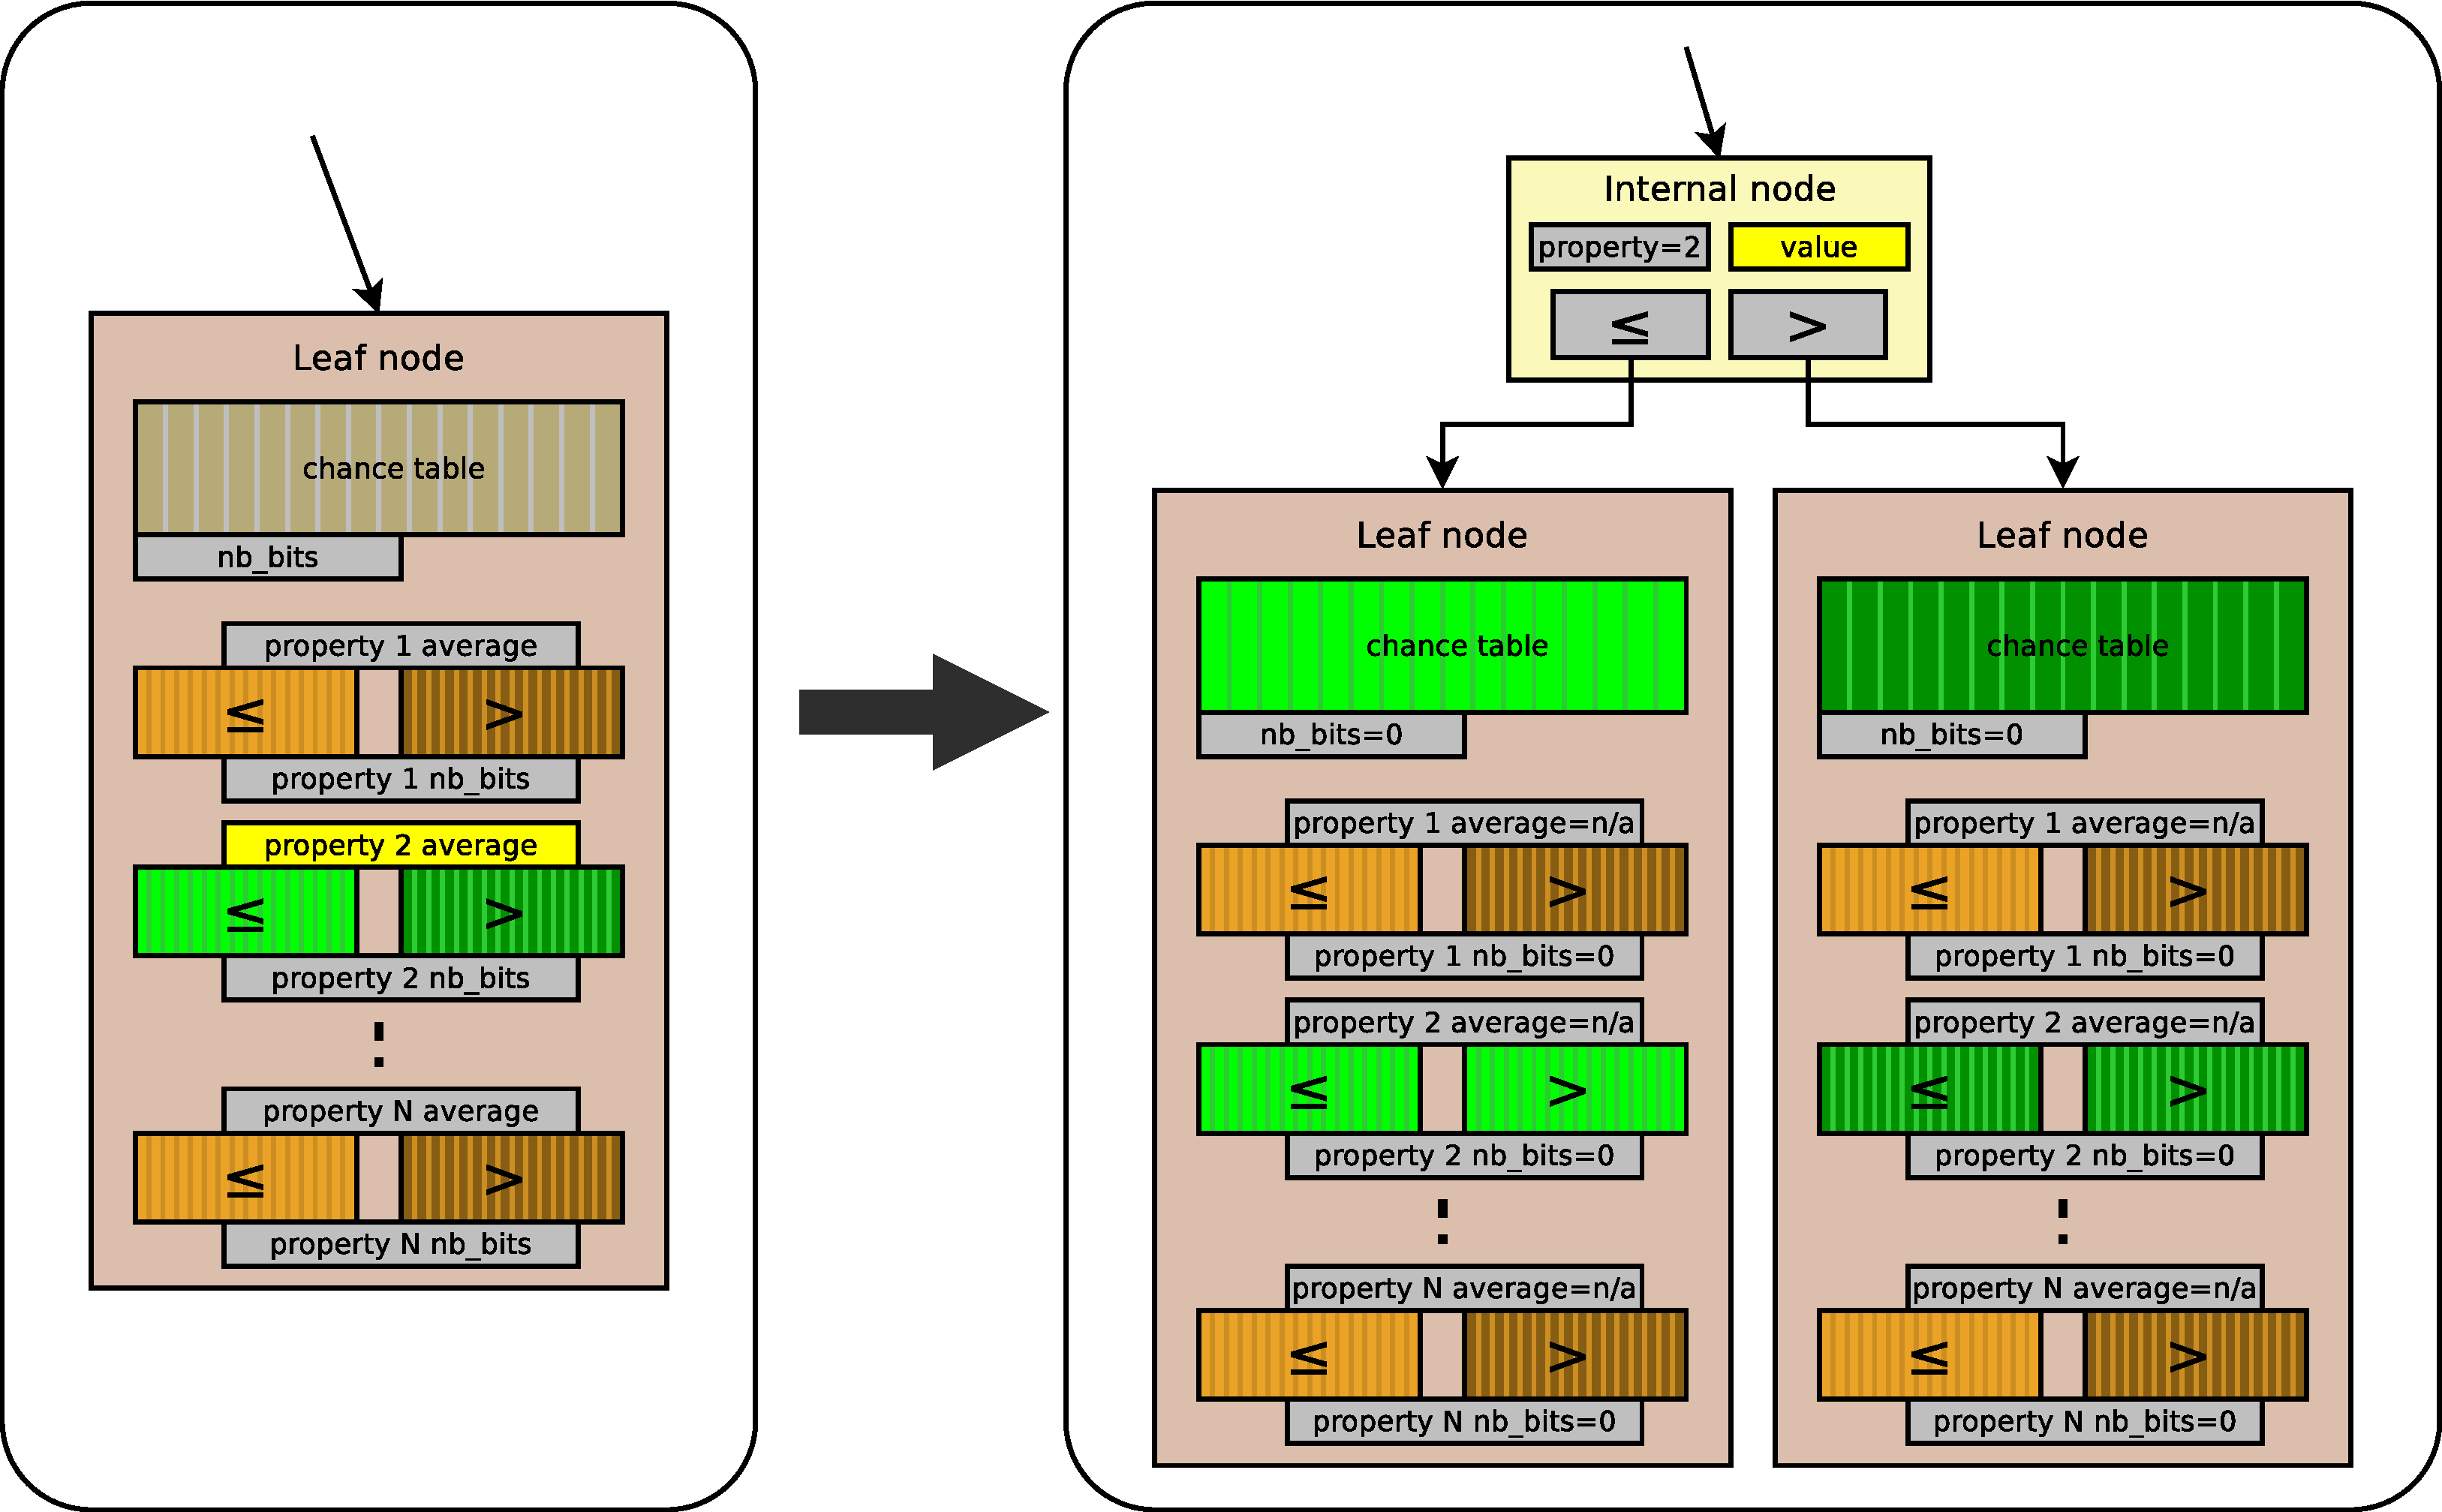
\includegraphics[width=\textwidth]{images/context_split}
\end{center}
\caption{Splitting on property 2, transforming one leaf node into an inner node and two new leaf nodes.}
\label{fig:context_tree_split}
\end{figure}

The context tree that we end up with is not necessarily the best one,
since it is constructed in a rather simplistic greedy way. However it does have three advantages compared
to using a fixed static context array:
\begin{itemize}
\item
There is no need to used quantized values for the properties, so if needed we can distinguish
between property values that are almost identical;
\item
The only properties that are actually used are those properties that turn out to contribute
to better compression for the given image;
\item
The size of the context tree (so the total number of contexts) depends on the given image,
the amount of pixels that are outputted and the actual relevance of the properties:
for a large, complex image,
more contexts will be used than for a small, simple image.
\end{itemize}



For brevity, we will call our method for entropy encoding ``MANIAC'', which stands for
Meta-Adaptive Near-zero Integer Arithmetic Coding. By ``meta-adaptive'', we mean the combination of
taking into account the output integer interval (see section~\ref{sec:rac:interval})
and in general, its domain of valid values (see section~\ref{sec:rac:bitvector}),
multiscale chance tables (see section~\ref{sec:multiscale}),
and, most importantly, the dynamic context tree learning (see section~\ref{sec:context_tree}).





\subsubsection{Two-pass Encoding}
Dynamic context tree learning can be done in a symmetric or asymmetric way.

In the symmetric method, encoding is done in a single pass. Trees are learned during encoding and do not need to be
part of the compressed file, since the decoder can construct the trees in the same way as the encoder -- all the information
needed is also available at decode time. As a result, encoding and decoding take roughly the same amount of time and space.

The main drawback of dynamically learning a context tree instead of using static contexts,
is the extra computational overhead arising from having to maintain the virtual contexts.
In fact, instead of doing the arithmetic coding once per pixel, it has to be done
up to $k+1$ times per pixel (where $k$ is the number of properties):
once for the ``actual'' context and up to $k$ times for the ``virtual'' contexts. The space needed per context
(to store the chance table and the bitcounts) goes from $O(1)$ to $O(1+2k)$.
However, there is a simple way to avoid the additional complexity during decoding.

In the asymmetric method, encoding is done in two (or more) passes.
In the first pass(es), we do exactly the same as before, except no actual compressed output is written.
The context trees are constructed and at the end, the final context trees are saved to the compressed file,
after some post-processing to simplify them. The actual chances and bitcounts are not saved, only the structure of the tree,
that is, the test in each node (one number to represent the property to test, another number to represent the value to compare to),
and also the number of times the node was visited as a leaf node, before it was ``split'' and became a decision node.\footnote{
This counter will be used to simulate the gradual reconstruction of the tree. Considering the tree as completely built from the start
leads to worse compression because then the chance tables are not initially shared and partially converged. However it does make sense
to make the counter smaller than its actual value (in the current implementation we divide it by a constant) because we already know
that the test ``will become useful in the future'' so it makes sense to ``split early''.}
In the second (last) pass, we consider the context trees
from the first pass(es) as given and proceed with normal encoding,
except that the context tree is already constructed so virtual contexts do not have to be maintained.
During decoding the context trees are read from the compressed file and decoding is quicker
because again there are no virtual contexts to maintain.

The compressed files can get slightly bigger than before
because we have to store the context trees and because we can no longer
use the best virtual context if it is better than the actual context.
However, the difference in compressed file size is relatively small while the
speedup for decoding can be significant.
Also, compression can be better if multiple passes are done, because that can lead to a better tree.
On typical images the cost of explicit trees is more than compensated by the gain from being able to use better trees.




\section{Experimental Evaluation} 
\label{sec:benchmarks}

In this section we evaluate the FLIF algorithm in terms of compression ratio.
We do this by comparison with other image compression algorithms:
PNG \cite{PNG}, lossless JPEG 2000 \cite{JPEG2000}, JPEG-LS \cite{JPEG-LS}, lossless WebP \cite{WebP},
lossless BPG, lossy JPEG \cite{JPEG} (at very high, near-lossless quality settings), and FFV1 \cite{FFV1}.
We will also compare ``lossy'' partial decodings of interlaced FLIF files
with progressive JPEG, progressive JPEG 2000, Adam7 interlaced PNG and interlaced GIF.
Finally we evaluate the time and space complexity of encoding and decoding.


\subsection{Compression Ratio}

The main aim of any compression algorithm is to get the best possible compression ratio.
The compression ratio is defined as the file size of the compressed image divided by the file size
of the uncompressed image --- lower is better.
In most cases, the uncompressed image uses 3 or 4 bytes per pixel (24 bit RGB or 32 bit RGBA).

[TODO: add benchmark results and discuss them]





\subsection{Computational Complexity}
\subsubsection{Time Complexity}

FLIF encoding has a log-linear $O(n \log n)$ time and space complexity (where $n$ is the number of pixels).
Decoding is also $O(n \log n)$. The logarithmic factor is due to the depth of the MANIAC trees, which has to be traversed to
find the leaf node. It can be reduced to a constant by imposing a depth limit on those trees if needed.

However, the constant factors hidden behind this notation are rather large.
In particular, if the MANIAC uses multiscaling with $k$ scales, and if there are $p$ properties, then every integer output or input
is done $(p+1)k$ times during encoding and $k$ times during decoding.





\subsubsection{Space Complexity}

The space complexity of FLIF is mostly influenced by the size of the image, the size of the context tree, and the size
of the color tables.

In the current implementation, the entire image is stored in memory --- in the case of FFV1-style image traversal,
it would be straightforward to reduce the space complexity by storing only two horizontal scanlines at a time;
in the case of recursive splitting it would be hard to avoid storing the entire image.

The size of the context tree can be controlled by adjusting the thresholds for enlarging the tree, or by simply
imposing a maximum tree size. In any case, the tree grows as the number of encoded pixels grows. For small images
(or easily compressible images), this means that the memory used for storing the context trees will be relatively small
(e.g. compared with FFV1).

The size of the color tables can be controlled by choosing the number of color buckets and the maximum
number of colors per discrete bucket.






\section{Conclusion and Future Work}
\label{sec:conclusion}

We have presented FLIF, which is a new image compression algorithm based on MANIAC entropy encoding.
It consistently outperforms existing standard compression algorithms like JPEG and PNG for lossless and near-lossless
compression; for medium-quality lossy compression of photographs, existing algorithms like JPEG 2000, WebP or BPG are still
a much better choice.
The main benefit of the FLIF image format is that it works well for both photographs and line art
(and combinations of those two), while the existing formats work well on only one of those categories (e.g. JPEG for photographs,
PNG for line art).




\subsection{Main Contributions}

MANIAC is a variant of arithmetic coding and can be applied not just to image compression. It is a general compression
method for integer numbers that are on average close to zero (e.g. differences between predicted and observed values).
MANIAC exploits all available information about the domain of the integers (e.g. in the case of FLIF, auto-indexing determines
the domain of the encoded integers). MANIAC also uses application-dependent context properties in such a way that
relevant properties are automatically exploited and irrelevant properties are ignored. Finally, because of
multiscaling, MANIAC automatically adjusts to the most appropriate time scale.

Some of the concepts used in FLIF are applicable more widely in other image processing and compression techniques.
We already mentioned MANIAC. Auto-indexing, a generalization of widely-used palette indexing, has many advantages compared
to traditional palette indexing. Most importantly, the combination of continuous and discrete color buckets means that no
arbitrary limit on the number of distinct colors has to be imposed, while the compression benefits of indexing can still be obtained.
Traditional palette indexing has the additional problem that the palette ordering heavily influences compression --- and since
the number of such orderings of $n$ colors is $n!$, exhaustive search for the optimal order is not feasible.
Auto-indexing does not have this problem; in this sense, it is more robust.




\subsection{Future Work}

The main idea behind the MANIAC is to use machine learning techniques to determine a relevant partitioning of the property space.
In a sense, we have used a very simple approach: we ``learn'' a decision tree (a rather simple kind of classifier),
where the learning is done in a very simple greedy way. More complicated classifiers and learning methods could be used.
Just like in the two-pass encoding mechanism,
learning does not need to be done on the fly. It does not necessarily have to be fast either --- encoding time is usually much less important
than decoding time. The only requirement is that the learned object (e.g. the decision tree) can be stored concisely and
that it can be reconstructed quickly during decoding.

Our current prototype only supports RGBA source images. In future work this should be extended to arbitrary data planes.
Our prototype does have preliminary support for animation; we will discuss this in a later paper.
Our choice to use YIQ color decomposition needs to be evaluated experimentally in order to
compare its compression performance to that of other color decompositions.



\bibliographystyle{plain}
\bibliography{biblio}

\end{document}
